% !TeX program = xelatex
\documentclass[a4paper,10pt]{article}

% ============================================================================
% ១. កញ្ចប់បណ្ណាល័យ និងការកំណត់ទំព័រ (Packages & Page Setup — តាមគំរូ ls_plan.tex)
% ============================================================================
\usepackage[a4paper, left=0.95cm, right=0.95cm, top=0.85cm, bottom=0.92cm, footskip=0.52cm]{geometry}
\usepackage{amsmath}
\usepackage{unicode-math}
\usepackage{fontspec}
\usepackage{longtable, array, multirow, colortbl}
\usepackage[table]{xcolor}
\usepackage{enumitem}
\usepackage{pifont}
\usepackage{fancyhdr}
\usepackage{tikz}
\usetikzlibrary{calc, arrows.meta, decorations.pathreplacing, patterns, positioning, babel}

\makeatletter
\let\@expl@@@mark@update@singlecol@structures@@\relax
\makeatother

% --- ប្រព័ន្ធស្វែងរកទីតាំងពុម្ពអក្សរស្វ័យប្រវត្តិ (Windows Local + Cloud Repo fonts/) ---
\providecommand{\NGSFindFonts}{%
  \IfFileExists{C:/Windows/Fonts/cambria.ttc}{%
    \def\NGSSysPath{C:/Windows/Fonts/}%
    \def\NGSUserPath{C:/Users/KIT/AppData/Local/Microsoft/Windows/Fonts/}%
  }{%
    \IfFileExists{./fonts/KhmerOSsiemreap.ttf}{\def\NGSSysPath{./fonts/}\def\NGSUserPath{./fonts/}}{%
    \IfFileExists{../fonts/KhmerOSsiemreap.ttf}{\def\NGSSysPath{../fonts/}\def\NGSUserPath{../fonts/}}{%
    \IfFileExists{../../fonts/KhmerOSsiemreap.ttf}{\def\NGSSysPath{../../fonts/}\def\NGSUserPath{../../fonts/}}{%
    \IfFileExists{../../../fonts/KhmerOSsiemreap.ttf}{\def\NGSSysPath{../../../fonts/}\def\NGSUserPath{../../../fonts/}}{%
    \IfFileExists{../../../../fonts/KhmerOSsiemreap.ttf}{\def\NGSSysPath{../../../../fonts/}\def\NGSUserPath{../../../../fonts/}}{%
    \IfFileExists{../../../../../fonts/KhmerOSsiemreap.ttf}{\def\NGSSysPath{../../../../../fonts/}\def\NGSUserPath{../../../../../fonts/}}{%
    \IfFileExists{../../../../../../fonts/KhmerOSsiemreap.ttf}{\def\NGSSysPath{../../../../../../fonts/}\def\NGSUserPath{../../../../../../fonts/}}{%
      \def\NGSSysPath{../../../../../../../fonts/}\def\NGSUserPath{../../../../../../../fonts/}%
    }}}}}}}%
  }%
}
\NGSFindFonts

% ============================================================================
% ២. កំណត់ពុម្ពអក្សរ (Fonts — តាមគំរូ ls_plan.tex)
% ============================================================================
\setmathfont[Path={\NGSSysPath}, FontIndex=1, Scale=1.02]{cambria.ttc}
\defaultfontfeatures{Ligatures=TeX}

\setmainfont[
  Path={\NGSUserPath},
  Extension=.ttf,
  Script=Khmer,
  BoldFont={KhmerOSsiemreap},
  BoldFeatures={FakeBold=1.8},
  ItalicFont={KhmerOSsiemreap},
  ItalicFeatures={FakeSlant=0.25},
  BoldItalicFont={KhmerOSsiemreap},
  BoldItalicFeatures={FakeBold=1.8, FakeSlant=0.25}
]{KhmerOSsiemreap}

\newfontfamily\muol[Path={\NGSUserPath}, Extension=.ttf, Script=Khmer]{KhmerOSmuollight}
\newfontfamily\Tacteing[Path={\NGSUserPath}, Extension=.TTF]{TACTENG}
\newfontfamily\TimesEn[Path={\NGSSysPath}, Extension=.ttf, BoldFont={timesbd}, ItalicFont={timesi}, BoldItalicFont={timesbi}]{times}
\newfontfamily\CalibriFont[Path={\NGSSysPath}, Extension=.ttf]{calibri}
\newfontfamily\CourierCirc[Path={\NGSSysPath}, Extension=.ttf]{cour}

\XeTeXlinebreaklocale "km"
\XeTeXlinebreakskip = 0pt plus 1pt minus 0.1pt

% ============================================================================
% ៣. ពណ៌ និងការតុបតែង (Colors & Styles)
% ============================================================================
\definecolor{stepbg}{HTML}{D9D9D9}
\definecolor{headgray}{HTML}{E6E6E6}
\definecolor{emphred}{HTML}{C00000}

\pagestyle{fancy}
\fancyhf{}
\renewcommand{\headrulewidth}{0pt}
\fancyfoot[R]{\CalibriFont\fontsize{9pt}{11pt}\selectfont\thepage}

\setlength{\parindent}{0pt}
\setlength{\parskip}{0pt}
\setlength{\tabcolsep}{4.5pt}
\setlength{\LTpre}{2pt}
\setlength{\LTpost}{2pt}

\newcolumntype{L}[1]{>{\raggedright\arraybackslash}p{#1}}
\newcolumntype{C}[1]{>{\centering\arraybackslash}p{#1}}

% ============================================================================
% ៤. ពាក្យបញ្ជាជំនួយ (Helper Macros)
% ============================================================================
\newcommand{\en}[1]{{\TimesEn #1}}
\newcommand{\enbf}[1]{{\TimesEn\bfseries #1}}
\newcommand{\khmflourish}{{\Tacteing\fontsize{15pt}{15pt}\selectfont 3}}
\newcommand{\wcirc}{{\CourierCirc\fontsize{9.5pt}{11pt}\selectfont o}}
\newcommand{\ditem}{{\fontsize{7.5pt}{10pt}\selectfont\ding{117}}\ }
\newcommand{\fiveE}[1]{\textcolor{emphred}{\CalibriFont\bfseries #1}}
\newcommand{\redsub}[1]{\textcolor{emphred}{#1}}
\newcommand{\timenote}[1]{\textcolor{emphred}{\textit{#1}}}
\newcommand{\stepheader}[1]{\multicolumn{3}{|c|}{\cellcolor{stepbg}\muol #1} \\ \hline}
\newcommand{\cfig}[1]{{\centering\vspace{3pt}#1\vspace{3pt}\par}}
\newcommand{\cnum}[1]{\mbox{\fontsize{10.5pt}{12pt}\selectfont\ding{\numexpr181+#1\relax}}}
\newcommand{\unit}[1]{\,\text{\en{#1}}}
\newcommand{\graybox}[1]{\colorbox{headgray}{\strut #1}}

% ============================================================================
% ៥. រូបភាព TikZ ស-ខ្មៅ សម្រាប់បង្រៀនលើក្ដារខៀន និងសន្លឹកកិច្ចការ (B&W Diagrams)
% ============================================================================

% ១. E1 Engage: អន្ទាក់ការបង្គត់ 15 824 យកត្រឹមខ្ទង់ពាន់ (ឧទាហរណ៍ ២ ទំ.១១)
\newcommand{\figEngageWNOneSix}{%
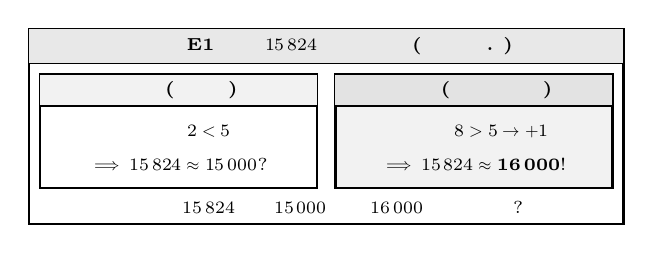
\begin{tikzpicture}[x=1cm, y=1cm, every node/.style={font=\fontsize{6.3pt}{8.3pt}\selectfont, text=black}]
  \draw[black, line width=0.9pt] (0,0) rectangle (7.55,2.48);
  \fill[gray!18] (0,2.04) rectangle (7.55,2.48);
  \draw[black, line width=0.6pt] (0,2.04) -- (7.55,2.04);
  \node at (3.775,2.26) {\textbf{បេសកកម្ម \en{E1}៖ បង្គត់ $15\,824$ យកត្រឹមខ្ទង់ពាន់ (ឧទាហរណ៍ ២ ទំ.១១)}};

  % Left: Student A
  \draw[black, line width=0.8pt] (0.14,0.46) rectangle (3.66,1.90);
  \fill[gray!10] (0.14,1.50) rectangle (3.66,1.90);
  \draw[black, line width=0.5pt] (0.14,1.50) -- (3.66,1.50);
  \node at (1.90,1.70) {\textbf{សិស្ស ក (មើលខុសខ្ទង់)}};
  \node at (1.90,1.18) {មើលខ្ទង់ដប់ $2 < 5$};
  \node at (1.90,0.76) {$\implies 15\,824 \approx 15\,000$?};

  % Right: Student B
  \draw[black, line width=0.95pt, fill=gray!10] (3.89,0.46) rectangle (7.41,1.90);
  \fill[gray!22] (3.89,1.50) rectangle (7.41,1.90);
  \draw[black, line width=0.55pt] (3.89,1.50) -- (7.41,1.50);
  \node at (5.65,1.70) {\textbf{សិស្ស ខ (មើលខ្ទង់រយជាប់ស្ដាំ)}};
  \node at (5.65,1.18) {មើលខ្ទង់រយ $8 > 5 \to +1$};
  \node at (5.65,0.76) {$\implies 15\,824 \approx \mathbf{16\,000}$!};

  \node at (3.775,0.21) {\textbf{សំណួរ៖} តើ $15\,824$ នៅជិត $15\,000$ ឬនៅជិត $16\,000$ ជាងលើបន្ទាត់ចំនួន?};
\end{tikzpicture}}

% ២. E2 Explore: បន្ទាត់ចំនួនធៀបចំណុចកណ្ដាល (ឧទាហរណ៍ ១ ទំ.១០៖ 647 និង 2931)
\newcommand{\figNumLineWNOneSix}{%
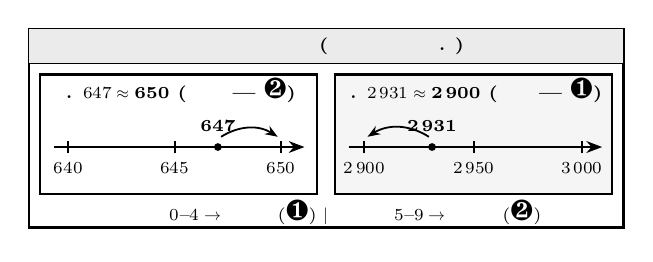
\begin{tikzpicture}[x=1cm, y=1cm, every node/.style={font=\fontsize{6.1pt}{8.0pt}\selectfont, text=black}]
  \draw[black, line width=0.9pt] (0,0) rectangle (7.55,2.52);
  \fill[gray!16] (0,2.08) rectangle (7.55,2.52);
  \draw[black, line width=0.6pt] (0,2.08) -- (7.55,2.08);
  \node at (3.775,2.30) {\textbf{បន្ទាត់ចំនួនធៀបចំណុចកណ្ដាល (ឧទាហរណ៍ ១ ក និង ខ ទំ.១០)}};

  % Left number line: 640 .. 645 .. 647 .. 650
  \draw[black, line width=0.8pt] (0.14,0.42) rectangle (3.66,1.94);
  \node at (1.90,1.74) {\textbf{ក. $647 \approx \mathbf{650}$ (ខ្ទង់ដប់ — \cnum{2})}};
  \draw[-{Stealth[length=2mm]}, black, line width=0.8pt] (0.32,1.02) -- (3.50,1.02);
  \draw[black, line width=0.7pt] (0.50,0.94) -- (0.50,1.10) node[below=4pt] {$640$};
  \draw[black, line width=0.7pt] (1.85,0.94) -- (1.85,1.10) node[below=4pt] {$645$};
  \fill[black] (2.40,1.02) circle (1.4pt) node[above=2pt] {$\mathbf{647}$};
  \draw[black, line width=0.7pt] (3.20,0.94) -- (3.20,1.10) node[below=4pt] {$650$};
  \draw[-{Stealth[length=1.6mm]}, black, bend left=32, line width=0.65pt] (2.44,1.15) to (3.16,1.15);

  % Right number line: 2900 .. 2931 .. 2950 .. 3000
  \draw[black, line width=0.8pt, fill=gray!8] (3.89,0.42) rectangle (7.41,1.94);
  \node at (5.65,1.74) {\textbf{ខ. $2\,931 \approx \mathbf{2\,900}$ (ខ្ទង់រយ — \cnum{1})}};
  \draw[-{Stealth[length=2mm]}, black, line width=0.8pt] (4.06,1.02) -- (7.28,1.02);
  \draw[black, line width=0.7pt] (4.26,0.94) -- (4.26,1.10) node[below=4pt] {$2\,900$};
  \fill[black] (5.12,1.02) circle (1.4pt) node[above=2pt] {$\mathbf{2\,931}$};
  \draw[black, line width=0.7pt] (5.65,0.94) -- (5.65,1.10) node[below=4pt] {$2\,950$};
  \draw[black, line width=0.7pt] (7.02,0.94) -- (7.02,1.10) node[below=4pt] {$3\,000$};
  \draw[-{Stealth[length=1.6mm]}, black, bend right=32, line width=0.65pt] (5.08,1.15) to (4.30,1.15);

  \node at (3.775,0.19) {លេខខាងស្ដាំ $0\text{--}4 \to$ បង្គត់ចុះ (\cnum{1}) $\mid$ លេខខាងស្ដាំ $5\text{--}9 \to$ បង្គត់ឡើង (\cnum{2})};
\end{tikzpicture}}

% ៣. E3 Explain: វិធានពិនិត្យលេខខាងស្ដាំបន្ទាប់ និងការប៉ាន់ស្មាន (ទំ.១០-១១)
\newcommand{\figRuleWNOneSix}{%
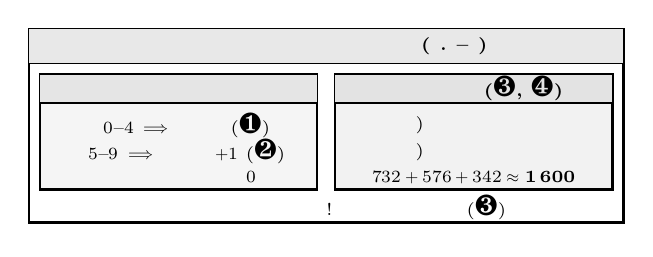
\begin{tikzpicture}[x=1cm, y=1cm, every node/.style={font=\fontsize{6.2pt}{8.1pt}\selectfont, text=black}]
  \draw[black, line width=0.9pt] (0,0) rectangle (7.55,2.46);
  \fill[gray!18] (0,2.02) rectangle (7.55,2.46);
  \draw[black, line width=0.6pt] (0,2.02) -- (7.55,2.02);
  \node at (3.775,2.24) {\textbf{វិធានបង្គត់តាមខ្ទង់ជាប់ស្ដាំ និងការប៉ាន់ស្មានចម្លើយ (ទំ.១០--១១)}};

  % Left box: Rounding rule
  \draw[black, line width=0.85pt, fill=gray!8] (0.14,0.42) rectangle (3.66,1.88);
  \fill[gray!20] (0.14,1.52) rectangle (3.66,1.88);
  \draw[black, line width=0.5pt] (0.14,1.52) -- (3.66,1.52);
  \node at (1.90,1.70) {\textbf{មើលលេខខាងស្ដាំជាប់ខ្ទង់គោលដៅ}};
  \node at (1.90,1.24) {បើ $0\text{--}4 \implies$ បង្គត់ចុះ (\cnum{1})};
  \node at (1.90,0.90) {បើ $5\text{--}9 \implies$ បង្គត់ឡើង $+1$ (\cnum{2})};
  \node at (1.90,0.58) {ជំនួសគ្រប់ខ្ទង់ខាងស្ដាំដោយលេខ $0$};

  % Right box: Estimation rule
  \draw[black, line width=0.85pt, fill=gray!10] (3.89,0.42) rectangle (7.41,1.88);
  \fill[gray!22] (3.89,1.52) rectangle (7.41,1.88);
  \draw[black, line width=0.5pt] (3.89,1.52) -- (7.41,1.52);
  \node at (5.65,1.70) {\textbf{ការប៉ាន់ស្មានចម្លើយ (\cnum{3}, \cnum{4})}};
  \node at (5.65,1.24) {១) បង្គត់តួនីមួយៗជាមុនសិន};
  \node at (5.65,0.90) {២) គណនាក្នុងចិត្តយ៉ាងរហ័ស};
  \node at (5.65,0.58) {$732+576+342 \approx \mathbf{1\,600}$};

  \node at (3.775,0.19) {\textbf{ប្រយ័ត្ន៖} កុំគណនាលេខធំប្រាកដមុនបង្គត់! ត្រូវបង្គត់ជាមុន ទើបគណនា (\cnum{3})};
\end{tikzpicture}}

% ៤. E4 Elaborate: លំហាត់គំរូទំ.១១ (870 x 38 : 95) និងត្រាទុកបន្តលើ 996 972
\newcommand{\figEstimateWNOneSix}{%
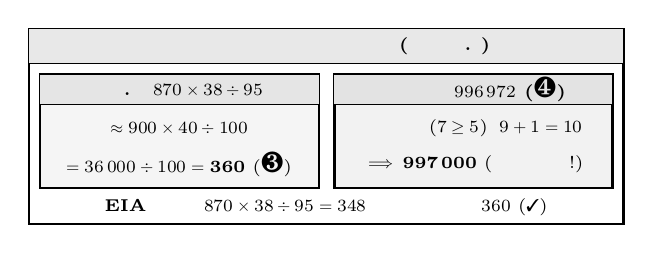
\begin{tikzpicture}[x=1cm, y=1cm, every node/.style={font=\fontsize{6.2pt}{8.2pt}\selectfont, text=black}]
  \draw[black, line width=0.9pt] (0,0) rectangle (7.55,2.48);
  \fill[gray!18] (0,2.04) rectangle (7.55,2.48);
  \draw[black, line width=0.6pt] (0,2.04) -- (7.55,2.04);
  \node at (3.775,2.26) {\textbf{លំហាត់គំរូប៉ាន់ស្មាន និងការបង្គត់មានត្រាទុកបន្ត (សៀវភៅគោល ទំ.១១)}};

  % Left: Model problem p.11
  \draw[black, line width=0.8pt, fill=gray!8] (0.14,0.46) rectangle (3.68,1.90);
  \fill[gray!20] (0.14,1.52) rectangle (3.68,1.90);
  \draw[black, line width=0.5pt] (0.14,1.52) -- (3.68,1.52);
  \node at (1.91,1.71) {\textbf{គំរូទំ.១១៖ $870 \times 38 \div 95$}};
  \node at (1.91,1.22) {$\approx 900 \times 40 \div 100$};
  \node at (1.91,0.76) {$= 36\,000 \div 100 = \mathbf{360}$ (\cnum{3})};

  % Right: Cascading carry 996 972
  \draw[black, line width=0.85pt, fill=gray!10] (3.88,0.46) rectangle (7.41,1.90);
  \fill[gray!22] (3.88,1.52) rectangle (7.41,1.90);
  \draw[black, line width=0.5pt] (3.88,1.52) -- (7.41,1.52);
  \node at (5.645,1.71) {\textbf{ប្រតិបត្តិ ខ៖ $996\,972$ (\cnum{4})}};
  \node at (5.645,1.22) {ត្រឹមខ្ទង់រយ ($7\ge 5$)៖ $9+1=10$};
  \node at (5.645,0.76) {$\implies \mathbf{997\,000}$ (ស្មើខ្ទង់ពាន់ដែរ!)};

  \node at (3.775,0.21) {\textbf{\en{EIA}៖} តម្លៃពិត $870\times 38\div 95 = 348$ ជិតនឹងតម្លៃប៉ាន់ស្មាន $360$ (\ding{51})};
\end{tikzpicture}}

% ៥. E5 Evaluate: សំណួរវិនិច្ឆ័យ A-D លើការបង្គត់ 49 962 ត្រឹមខ្ទង់រយ
\newcommand{\figExitWNOneSix}{%
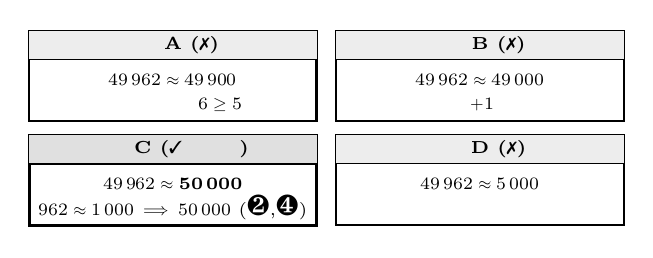
\begin{tikzpicture}[x=1cm, y=1cm, every node/.style={font=\fontsize{6.3pt}{8.2pt}\selectfont, text=black}]
  % Choice A
  \draw[black, line width=0.8pt] (0,1.32) rectangle (3.65,2.46);
  \fill[gray!14] (0,2.10) rectangle (3.65,2.46);
  \draw[black, line width=0.5pt] (0,2.10) -- (3.65,2.10);
  \node at (1.825,2.28) {\textbf{ជម្រើស \en{A} (\ding{55})}};
  \node at (1.825,1.84) {$49\,962 \approx 49\,900$};
  \node at (1.825,1.53) {ច្រឡំបង្គត់ចុះទាំង $6 \ge 5$};

  % Choice B
  \draw[black, line width=0.8pt] (3.90,1.32) rectangle (7.55,2.46);
  \fill[gray!14] (3.90,2.10) rectangle (7.55,2.46);
  \draw[black, line width=0.5pt] (3.90,2.10) -- (7.55,2.10);
  \node at (5.725,2.28) {\textbf{ជម្រើស \en{B} (\ding{55})}};
  \node at (5.725,1.84) {$49\,962 \approx 49\,000$};
  \node at (5.725,1.53) {ភ្លេចត្រាទុក $+1$ ទៅខ្ទង់ពាន់};

  % Choice C (Correct)
  \draw[black, line width=1.05pt] (0,0) rectangle (3.65,1.14);
  \fill[gray!24] (0,0.78) rectangle (3.65,1.14);
  \draw[black, line width=0.6pt] (0,0.78) -- (3.65,0.78);
  \node at (1.825,0.96) {\textbf{ជម្រើស \en{C} (\ding{51} ត្រឹមត្រូវ)}};
  \node at (1.825,0.52) {$49\,962 \approx \mathbf{50\,000}$};
  \node at (1.825,0.22) {$962 \approx 1\,000 \implies 50\,000$ (\cnum{2},\cnum{4})};

  % Choice D
  \draw[black, line width=0.8pt] (3.90,0) rectangle (7.55,1.14);
  \fill[gray!14] (3.90,0.78) rectangle (7.55,1.14);
  \draw[black, line width=0.5pt] (3.90,0.78) -- (7.55,0.78);
  \node at (5.725,0.96) {\textbf{ជម្រើស \en{D} (\ding{55})}};
  \node at (5.725,0.52) {$49\,962 \approx 5\,000$};
  \node at (5.725,0.22) {សរសេរបាត់លេខសូន្យ ១ ខ្ទង់};
\end{tikzpicture}}

\begin{document}
\fontsize{10pt}{15.2pt}\selectfont

% ============================================================================
% ក្បាលរដ្ឋបាល (Administrative Header — តាមគំរូ ls_plan.tex)
% ============================================================================
{\centering
  {\muol\fontsize{11pt}{16pt}\selectfont ព្រះរាជាណាចក្រកម្ពុជា\par}
  {\muol\fontsize{11pt}{16pt}\selectfont ជាតិ សាសនា ព្រះមហាក្សត្រ\par}
  \vspace{-3pt}{\khmflourish\par}
}

\vspace{1pt}
{\muol\fontsize{10pt}{15.5pt}\selectfont
មន្ទីរអប់រំ យុវជន និងកីឡា ខេត្តកំពង់ធំ\par
ការិយាល័យអប់រំ យុវជន និងកីឡា ស្រុកកំពង់ស្វាយ\par
អនុវិទ្យាល័យព្រះក្រសាំង\par}

\vspace{2pt}
{\centering{\muol\fontsize{11.5pt}{17pt}\selectfont កិច្ចតែងការបង្រៀន\par}}
\vspace{2pt}

% --- ព័ត៌មានទូទៅ ---
{\hspace*{2.8cm}\renewcommand{\arraystretch}{1.08}
\begin{tabular}{@{}l@{\hspace{0.35cm}}p{2.9cm}@{\hspace{0.15cm}}c@{\hspace{0.25cm}}l@{}}
  - & មុខវិជ្ជា & : & គណិតវិទ្យា ថ្នាក់ទី៧ (ពីជគណិត) \\
  - & ចំណងជើងមេរៀន & : & មេរៀនទី១៖ ចំនួនគត់ \\
  - & ចំណងជើងរង & : & ៧. ការបង្គត់ចំនួនគត់ និងការប៉ាន់ស្មាន (ទំ.១០--១១) \\
  - & រយៈពេល & : & ១ ម៉ោងសិក្សា (៥០ នាទី) \\
  - & បង្រៀនដោយ & : & ហុក ប៊ុនថែន \\
  - & កាលបរិច្ឆេទ & : & ថ្ងៃអង្គារ ទី១០ ខែវិច្ឆិកា ឆ្នាំ២០២៦ \\
\end{tabular}\par}

\vspace{2pt}

% --- I. វត្ថុបំណង ---
{\muol\fontsize{10pt}{15.5pt}\selectfont \enbf{I.} វត្ថុបំណង\par}
\vspace{1pt}
{\renewcommand{\arraystretch}{1.10}
\begin{tabular}{@{}p{0.55cm}@{}p{2.35cm}@{\hspace{0.15cm}}c@{\hspace{0.25cm}}p{14.95cm}@{}}
  \hfill\wcirc\hspace{0.2cm} & វិជ្ជាសម្បទា & : & សិស្សប្រាប់បានពីវិធានបង្គត់ចំនួនគត់យកត្រឹមខ្ទង់ដប់ ខ្ទង់រយ និងខ្ទង់ពាន់ (ពិនិត្យលេខខាងស្ដាំជាប់ខ្ទង់គោលដៅ៖ $0\text{--}4$ បង្គត់ចុះ និង $5\text{--}9$ បង្គត់ឡើង) ព្រមទាំងន័យនៃការប៉ាន់ស្មានចម្លើយបានត្រឹមត្រូវ ។ \\
  \hfill\wcirc\hspace{0.2cm} & បំណិនសម្បទា & : & សិស្សបង្គត់ចំនួនគត់ធំៗ (រួមទាំងករណីត្រាទុកបន្តលើលេខ $9$) និងប៉ាន់ស្មានតម្លៃនៃផលបូក ផលគុណ និងផលចែកដោយបង្គត់ជាមុនលើសន្លឹកកិច្ចការបានត្រឹមត្រូវ ។ \\
  \hfill\wcirc\hspace{0.2cm} & ចរិយាសម្បទា & : & សិស្សមានទម្លាប់ប្រើការប៉ាន់ស្មានដើម្បីត្រួតពិនិត្យភាពសមហេតុផលនៃចម្លើយក្នុងជីវភាពប្រចាំថ្ងៃ មានភាពហ្មត់ចត់លើចំនួនលេខសូន្យខាងស្ដាំ និងសហការគ្នាជាក្រុម ។ \\
\end{tabular}\par}

\vspace{2pt}

% --- II. សម្ភារៈឧបទេស ---
{\muol\fontsize{10pt}{15.5pt}\selectfont \enbf{II.} សម្ភារៈឧបទេស\par}
\vspace{1pt}
\hspace*{0.55cm}$\bullet$\ សៀវភៅសិក្សាគោលថ្នាក់ទី៧ (ទំ.១០--១១ និងទំ.១៤) ក្ដារខៀន ដីស/ហ្វឺត បន្ទាត់ត្រង់ និង\textbf{សន្លឹកកិច្ចការសិស្សបំពេញចន្លោះ ស-ខ្មៅ} (កូដ \en{WN16} ទំព័រ ១--២ សម្រាប់សិស្ស និងទំព័រ ៣ ប្លង់ក្ដារខៀន/ចម្លើយគ្រូ — គ្មានប្រើ \en{LCD})\par

\vspace{2pt}

% --- III. វិធីសាស្រ្តបង្រៀន ---
{\muol\fontsize{10pt}{15.5pt}\selectfont \enbf{III.} វិធីសាស្រ្តបង្រៀន\par}
\vspace{1pt}
{\renewcommand{\arraystretch}{1.08}
\begin{tabular}{@{}p{0.55cm}@{}p{2.35cm}@{\hspace{0.15cm}}c@{\hspace{0.25cm}}p{14.95cm}@{}}
  \hfill$\bullet$\hspace{0.2cm} & គោលវិធី & : & សិស្សមជ្ឈមណ្ឌល (សន្លឹកកិច្ចការបំពេញចន្លោះជាគោល + ការពិភាក្សាជាក្រុមតូច ៣ នាក់) \\
  \hfill$\bullet$\hspace{0.2cm} & យុទ្ធវិធីបង្រៀន & : & គំរូស្ថាបនានិយម \en{5Es} រួមបញ្ចូល \textbf{បន្ទាត់ចំនួនធៀបចំណុចកណ្ដាល (\en{Midpoint Number-Line Benchmark})} និង \textbf{ការប៉ាន់ស្មានដោយលេខស៊ីគ្នា (\en{Compatible-Number Estimation})} \\
\end{tabular}\par}

\vspace{2pt}

% --- IV. ដំណើរការបង្រៀន ---
{\muol\fontsize{10pt}{15.5pt}\selectfont \enbf{IV.} ដំណើរការបង្រៀន\par}

{\renewcommand{\arraystretch}{1.15}
\begin{longtable}{|L{5.50cm}|L{7.90cm}|L{4.80cm}|}
\hline
\multicolumn{1}{|c|}{\cellcolor{headgray}\muol សកម្មភាពគ្រូ} &
\multicolumn{1}{c|}{\cellcolor{headgray}\muol ខ្លឹមសារមេរៀន} &
\multicolumn{1}{c|}{\cellcolor{headgray}\muol សកម្មភាពសិស្ស} \\
\hline
\endfirsthead

\hline
\multicolumn{1}{|c|}{\cellcolor{headgray}\muol សកម្មភាពគ្រូ} &
\multicolumn{1}{c|}{\cellcolor{headgray}\muol ខ្លឹមសារមេរៀន} &
\multicolumn{1}{c|}{\cellcolor{headgray}\muol សកម្មភាពសិស្ស} \\
\hline
\endhead

% ==================== ជំហានទី១ (2min) ====================
\stepheader{ជំហានទី១ \enbf{(}រដ្ឋបាលថ្នាក់\enbf{)}}
$\bullet$ ពិនិត្យវត្តមាន អនាម័យ និងសណ្ដាប់ធ្នាប់ថ្នាក់រៀន \par
$\bullet$ រៀបចំក្រុមតូច ៣ នាក់តាមតុ និងចែក\textbf{សន្លឹកកិច្ចការសិស្ស (\en{WN16} ទំព័រ ១–២)}
&
$\bullet$ រដ្ឋបាលថ្នាក់ អនាម័យ និងវិន័យសិក្សា \par
$\bullet$ ចែកសន្លឹកកិច្ចការម្នាក់ ១ សន្លឹក សម្រាប់បំពេញតាមដំណាក់កាល \en{E1--E5}
&
$\circ$ ប្រធានថ្នាក់រាយការណ៍វត្តមានសិស្ស \par
$\circ$ ទទួលសន្លឹកកិច្ចការ សរសេរឈ្មោះ និងអង្គុយតាមក្រុម ៣ នាក់ \\
\hline

% ==================== ជំហានទី២ (9min: កំណែ <=3m + រំលឹក 3m + E1 3m) ====================
\stepheader{ជំហានទី២ \enbf{(}កិច្ចការផ្ទះ \enbf{+} ទំនាក់ទំនងមេរៀនថ្មី\enbf{)}}
\ditem \textbf{កំណែកិច្ចការផ្ទះ ($\le\text{\enbf{3\,min}}$)} \par
$\bullet$ ហៅសិស្សឡើងកែលំហាត់ទំ.១៤ លេខ ២ (ខ, គ, ឃ, ង) លើក្ដារខៀនផ្នែកឆ្វេង
&
{\centering\redsub{កំណែកិច្ចការផ្ទះមេរៀនមុន (ទំ.១៤ លេខ ២ ខ, គ, ឃ, ង)}\par}
$\bullet$ \textbf{ខ.} $65\times 20 + 360 = \mathbf{1\,660}$ \quad $\bullet$ \textbf{គ.} $7 + 6 - 13 = \mathbf{0}$ \par
$\bullet$ \textbf{ឃ.} $[69 - 4]\times 2 = \mathbf{130}$ \quad $\bullet$ \textbf{ង.} $75 - 19 + 105 + 21 - 15 + 42 = \mathbf{209}$
&
$\circ$ ផ្ទៀងចម្លើយ ($1\,660; 0; 130; 209$) និងកែតម្រូវចូលសៀវភៅ \\[3pt]

\ditem \textbf{រំលឹកមេរៀនទាក់ទង (\enbf{3min})} \par
$\bullet$ សួរ៖ «ក្នុងចំនួន $15\,824$ តើលេខណាឈរនៅខ្ទង់ពាន់ ហើយលេខណានៅខាងស្ដាំជាប់ខ្ទង់ពាន់?»
&
{\centering\redsub{រំលឹកតម្លៃតាមខ្ទង់ និងចំណុចកណ្ដាលលើបន្ទាត់ចំនួន}\par}
$\bullet$ ក្នុង $15\,824$៖ លេខ $5$ ឈរនៅ\textbf{ខ្ទង់ពាន់} ហើយលេខ $8$ ឈរនៅ\textbf{ខ្ទង់រយ} (ខាងស្ដាំជាប់ខ្ទង់ពាន់)
&
$\circ$ ឆ្លើយ៖ «លេខ $5$ នៅខ្ទង់ពាន់ និងលេខ $8$ នៅខាងស្ដាំជាប់វា!» \\[3pt]

$\bullet$ សួរបន្ត៖ «រវាង $640$ និង $650$ តើចំនួនគត់មួយណាស្ថិតនៅចំកណ្ដាល?»
&
$\bullet$ ចំណុចកណ្ដាលរវាង $640$ និង $650$ គឺ $645$ (រីឯរវាង $2\,900$ និង $3\,000$ គឺ $2\,950$)
&
$\circ$ ឆ្លើយ៖ «$645$ និង $2\,950$ ជាចំណុចកណ្ដាល!» \\[3pt]

\fiveE{E1 - Engage (3min)} \timenote{(កុំទាន់ផ្ដល់ចម្លើយ)} \par
\ditem \textbf{បេសកកម្មអន្ទាក់ការបង្គត់ត្រឹមខ្ទង់ពាន់ (សន្លឹកកិច្ចការ \en{E1})} \par
$\bullet$ ឱ្យសិស្សពិនិត្យប្រអប់ \en{E1} លើការបង្គត់ $15\,824$ យកត្រឹមខ្ទង់ពាន់ (ឧទាហរណ៍ ២ ទំ.១១)
&
\redsub{បេសកកម្ម \en{E1}៖ បង្គត់ $15\,824$ យកត្រឹមខ្ទង់ពាន់ (ទំ.១១)} \par
$\bullet$ \textbf{សិស្ស ក} មើលខ្ទង់ដប់ ($2 < 5$) បង្គត់ជា $15\,000$ \par
$\bullet$ \textbf{សិស្ស ខ} មើលខ្ទង់រយ ($8 > 5$) បង្គត់ជា $16\,000$ ។ តើអ្នកណាត្រឹមត្រូវ?
&
$\circ$ ពិភាក្សាជាគូ និងគូស \ding{51} ក្នុងប្រអប់ \en{E1} លើសន្លឹកកិច្ចការ \\[3pt]

&
\cfig{\figEngageWNOneSix}
& \\
\hline

% ==================== ជំហានទី៣ (17min: E2 11m + E3 6m) ====================
\stepheader{ជំហានទី៣ \enbf{(}ខ្លឹមសារមេរៀនថ្មី\enbf{)}}
\fiveE{E2 - Explore (11min)} \par
$\bullet$ សរសេរចំណងជើងរង \textbf{៧. ការបង្គត់ចំនួនគត់ និងការប៉ាន់ស្មាន} លើក្ដារខៀន \par
\ditem \textbf{សកម្មភាព ១៖ បន្ទាត់ចំនួនធៀបចំណុចកណ្ដាល (ឧទាហរណ៍ ១ ទំ.១០, \enbf{5min}, \en{E2-A})} \par
$\bullet$ ឱ្យសិស្សដៅចំណុច $647$ និង $2\,931$ លើបន្ទាត់ចំនួនក្នុង \en{E2-A} រួចសន្និដ្ឋានការបង្គត់
&
៧. ការបង្គត់ចំនួនគត់ និងការប៉ាន់ស្មាន \par
$\bullet$ \textbf{ឧទាហរណ៍ ១ ក (ទំ.១០)៖} $647$ នៅជិត $650$ ជាង $640 \implies 647 \approx \mathbf{650}$ (ត្រឹមខ្ទង់ដប់) \par
$\bullet$ \textbf{ឧទាហរណ៍ ១ ខ (ទំ.១០)៖} $2\,931$ នៅជិត $2\,900$ ជាង $3\,000 \implies 2\,931 \approx \mathbf{2\,900}$ (ខ្ទង់រយ)
&
$\circ$ ដៅចំណុចលើបន្ទាត់ចំនួន និងបំពេញ $650$ និង $2\,900$ \\[3pt]

&
\cfig{\figNumLineWNOneSix}
& \\[3pt]

\ditem \textbf{សកម្មភាព ២៖ ការពិនិត្យលេខខាងស្ដាំ និងការប៉ាន់ស្មានផលបូក (ទំ.១១, \enbf{6min}, \en{E2-B})} \par
$\bullet$ ឱ្យសិស្សបង្គត់ $15\,824$ ត្រឹមខ្ទង់រយ និងត្រឹមខ្ទង់ពាន់លើ \en{E2-B} (\emph{កែលេខពុម្ពទំ.១១ «$1\,6\,0\,0$»})
&
$\bullet$ \textbf{ឧទាហរណ៍ ២ (ទំ.១១)៖} ចំនួន $15\,824$ \par
\hspace*{0.2cm}១) ត្រឹមខ្ទង់រយ (មើលខ្ទង់ដប់ $2 < 5$) $\to \mathbf{15\,800}$ \par
\hspace*{0.2cm}២) ត្រឹមខ្ទង់ពាន់ (មើលខ្ទង់រយ $8 > 5$) $\to \mathbf{16\,000}$ (\emph{កែលេខពុម្ពទំ.១១ ដែលបាត់សូន្យមួយ})
&
$\circ$ គូសព្រួញមើលខ្ទង់ជាប់ស្ដាំ ឃើញ $15\,800$ និង $16\,000$ \\[3pt]

$\bullet$ ឱ្យសិស្សប៉ាន់ស្មានផលបូក $732 + 576 + 342$ (ឧទាហរណ៍ទំ.១១) ដោយបង្គត់ត្រឹមខ្ទង់រយជាមុន
&
$\bullet$ \textbf{ឧទាហរណ៍ការប៉ាន់ស្មាន (ទំ.១១)៖} \par
\hspace*{0.2cm}$732 + 576 + 342 \approx 700 + 600 + 300 = \mathbf{1\,600}$ (\emph{កែលេខពុម្ពទំ.១១ «$16.000$» ជា «$1\,600$»})
&
$\circ$ បង្គត់ជា $700+600+300$ គណនាក្នុងចិត្តឃើញ $1\,600$ \\[3pt]

% --- E3 Explain (6min) ---
\fiveE{E3 - Explain (6min)} \par
$\bullet$ ដឹកនាំសិស្សសង្ខេបវិធានបង្គត់ជាទូទៅ និងវិធានប៉ាន់ស្មាន (ទំ.១០--១១) លើ \en{E3}
&
$\bullet$ \textbf{វិធានជាទូទៅ (ទំ.១០--១១)៖} មើលតែលេខ\textbf{មួយខ្ទង់នៅខាងស្ដាំជាប់ខ្ទង់ដែលចង់បង្គត់}៖ \par
\hspace*{0.15cm}១) បើជាលេខ \graybox{$0$ ដល់ $4$} ត្រូវ\textbf{បង្គត់ចុះ} (រក្សាខ្ទង់គោលដៅ ជំនួសខ្ទង់ស្ដាំដោយ $0$) \par
\hspace*{0.15cm}២) បើជាលេខ \graybox{$5$ ដល់ $9$} ត្រូវ\textbf{បង្គត់ឡើង} (បន្ថែម $+1$ លើខ្ទង់គោលដៅ ជំនួសខ្ទង់ស្ដាំដោយ $0$)
&
$\circ$ បំពេញប្រអប់វិធានបង្គត់ចុះនិងបង្គត់ឡើងលើ \en{E3} \\[3pt]

$\bullet$ ភ្ជាប់\textbf{ធនាគារហេតុផល \cnum{1}--\cnum{2}} លើក្ដារខៀន និងសន្លឹកកិច្ចការ
&
\textbf{ធនាគារហេតុផល (\en{Warrant Bank})៖} \par
\cnum{1} \textbf{បង្គត់ចុះ ($<5$)៖} លេខខាងស្ដាំ $0\text{--}4 \to$ រក្សាខ្ទង់គោលដៅ ជំនួសស្ដាំដោយ $0$ \par
\cnum{2} \textbf{បង្គត់ឡើង ($\ge 5$)៖} លេខខាងស្ដាំ $5\text{--}9 \to$ បូក $+1$ លើខ្ទង់គោលដៅ ជំនួសស្ដាំដោយ $0$
&
$\circ$ ផ្ទៀងលេខកូដ \cnum{1}--\cnum{2} លើសន្លឹកកិច្ចការ \\[3pt]

$\bullet$ ភ្ជាប់\textbf{ធនាគារហេតុផល \cnum{3}--\cnum{4}} សម្រាប់ការប៉ាន់ស្មាន និងការត្រាទុកបន្តលើលេខ $9$
&
\cnum{3} \textbf{ប៉ាន់ស្មានរហ័ស៖} បង្គត់តួនីមួយៗជាមុនសិន រួចទើបគណនា ($\approx$) \par
\cnum{4} \textbf{ត្រាទុក $9+1=10$៖} បន្ថែម $+1$ បន្តទៅខ្ទង់ខាងឆ្វេងបន្ទាប់
&
$\circ$ ផ្ទៀងលេខកូដ \cnum{3}--\cnum{4} លើសន្លឹកកិច្ចការ \\[3pt]

&
\cfig{\figRuleWNOneSix}
& \\
\hline

% ==================== ជំហានទី៤ (20min: E4 10m + E5 10m) ====================
\stepheader{ជំហានទី៤ \enbf{(}ពង្រីកចំណេះដឹង\enbf{)}}
\fiveE{E4 - Elaborate (10min)} \par
\ditem \textbf{លំហាត់គំរូ៖ ការប៉ាន់ស្មានចម្លើយប្រមាណវិធីចម្រុះ (សៀវភៅគោល ទំ.១១)} \par
$\bullet$ ឱ្យសិស្សប៉ាន់ស្មានកន្សោម $870 \times 38 \div 95$ តាមជំហានបង្គត់មុនគណនាលើ \en{E4}
&
{\muol លំហាត់គំរូ} \textbf{(ទំ.១១ — ធ្វើការប៉ាន់ស្មានចម្លើយនៃ $870 \times 38 \div 95$)៖} \par
$\bullet$ បង្គត់តួនីមួយៗ៖ $870 \approx 900$, \quad $38 \approx 40$, \quad $95 \approx 100$ \par
$\bullet$ គណនាក្នុងចិត្ត (\cnum{3})៖ $900 \times 40 \div 100 = 36\,000 \div 100 = \graybox{$360$}$
&
$\circ$ បង្គត់ជា $900\times 40\div 100$ គណនាឃើញប្រហែល $360$ \\[3pt]

&
\cfig{\figEstimateWNOneSix}
& \\[3pt]

$\bullet$ សួរសំណួរឆ្លុះបញ្ចាំង \textbf{\en{EIA Looking-Back} (1min)} ប្រៀបធៀបតម្លៃប៉ាន់ស្មាននឹងតម្លៃពិត
&
\textbf{\en{EIA Looking-Back}៖} «តម្លៃប្រាកដនៃ $870\times 38\div 95$ គឺ $348$ ។ បើសិស្សម្នាក់គណនាខុសខ្ទង់ឃើញ $3\,480$ តើការប៉ាន់ស្មាន $360$ ជួយចាប់កំហុសបានភ្លាមដូចម្ដេច?» ($\to 3\,480$ ខុសឆ្ងាយពី $360$ ដល់ទៅ $10$ ដង!)
&
$\circ$ យល់ពីអត្ថប្រយោជន៍នៃការប៉ាន់ស្មានដើម្បីចាប់កំហុសរំកិលខ្ទង់ \\[3pt]

% --- E5 Evaluate (10min) ---
\fiveE{E5 - Evaluate (10min)} \par
\ditem \textbf{ប្រតិបត្តិជាក្រុមតូច ៣ នាក់ (4min, សន្លឹកកិច្ចការ \en{E5})} \par
$\bullet$ ឱ្យក្រុមសិស្សបំពេញតារាងបង្គត់លំហាត់ប្រតិបត្តិទំ.១១ (ក, ខ, គ) យកត្រឹមខ្ទង់ដប់ រយ និងពាន់
&
{\muol លំហាត់ប្រតិបត្តិ} \textbf{(ទំ.១១ — បង្គត់ត្រឹមខ្ទង់ដប់ ខ្ទង់រយ និងខ្ទង់ពាន់)៖} \par
$\bullet$ \textbf{ក.} $7\,663\,692 \to \mathbf{7\,663\,690}; \ \mathbf{7\,663\,700}; \ \mathbf{7\,664\,000}$ \par
$\bullet$ \textbf{ខ.} $996\,972 \to \mathbf{996\,970}; \ \mathbf{997\,000}$ (\cnum{4}); $\mathbf{997\,000}$ \quad \textbf{គ.} $3\,500\,004 \to \mathbf{3\,500\,000}$ (ទាំងបី)
&
$\circ$ សហការគ្នាបំពេញតារាងបង្គត់ទាំង ៩ ប្រអប់បានត្រឹមត្រូវ \\[3pt]

$\bullet$ ឱ្យក្រុមសិស្សផ្ទៀងផ្ទាត់និង\textbf{បិទបេសកកម្ម \en{E1} (2min)}
&
$\bullet$ \textbf{បិទបេសកកម្ម \en{E1}៖} \textbf{សិស្ស ខ} ត្រឹមត្រូវ! $15\,824 \approx \mathbf{16\,000}$ (\cnum{2}) ព្រោះខ្ទង់រយនៅខាងស្ដាំជាប់ខ្ទង់ពាន់គឺ $8 \ge 5$ ។
&
$\circ$ បិទបេសកកម្ម \en{E1} ឃើញសិស្ស ខ ត្រឹមត្រូវ ($16\,000$) \\[3pt]

\ditem \textbf{សំណួរវិនិច្ឆ័យ \en{A--D} និងសំបុត្រចេញ (4min)} \par
$\bullet$ សរសេរលំហាត់បង្គត់ $49\,962$ យកត្រឹមខ្ទង់រយ និងជម្រើស \en{A--D} លើក្ដារខៀន
&
{\centering\textbf{សំណួរវិនិច្ឆ័យ \en{A--D}៖ បង្គត់ចំនួន $49\,962$ យកត្រឹមខ្ទង់រយ តើស្មើនឹងប៉ុន្មាន?}\par}
&
$\circ$ ពិនិត្យខ្ទង់ដប់ $6 \ge 5$ និងត្រាទុក $9+1=10$ បន្តទៅម៉ឺន \\[3pt]

$\bullet$ ឱ្យសិស្សគូសរង្វង់ជម្រើសត្រូវលើសន្លឹកកិច្ចការ រួចលើកម្រាមដៃ ១--៤ ព្រមគ្នា \par
$\bullet$ ហៅសិស្សបកស្រាយហេតុផលដែលជម្រើស \en{A}, \en{B} និង \en{D} ខុស
&
$\bullet$ វិភាគកំហុសក្នុងជម្រើសនីមួយៗតាមលេខកូដហេតុផល \cnum{2} និង \cnum{4}៖ \par
\hspace*{0.15cm}-- ជម្រើស \en{A} ($49\,900$)៖ ខុសព្រោះបង្គត់ចុះទាំងខ្ទង់ដប់គឺ $6 \ge 5$ \par
\hspace*{0.15cm}-- ជម្រើស \en{B} ($49\,000$) និង \en{D} ($5\,000$)៖ ខុសព្រោះភ្លេចត្រាទុក ឬបាត់សូន្យ
&
$\circ$ គូសរង្វង់លើសន្លឹកកិច្ចការ និងលើកម្រាមដៃ ៣ (\textbf{ជម្រើស \en{C}}) \par
$\circ$ បកស្រាយការត្រាទុកបន្ត $962 \approx 1\,000 \implies 50\,000$ \\[3pt]

&
\cfig{\figExitWNOneSix}
& \\[3pt]

$\bullet$ បញ្ជាក់ចម្លើយត្រូវ (\textbf{ជម្រើស \en{C}}) និងឱ្យបំពេញ\textbf{សំបុត្រចេញ ៦០ វិនាទី}
&
$\bullet$ \textbf{សំបុត្រចេញ៖} ប៉ាន់ស្មាន $592 \times 41 \approx 600 \times 40 = \mathbf{24\,000}$ (\cnum{3}) ។
&
$\circ$ បំពេញសំបុត្រចេញឃើញប្រហែល $24\,000$ មុនបញ្ចប់ម៉ោង \\
\hline

% ==================== ជំហានទី៥ (<=2min) ====================
\stepheader{ជំហានទី៥ \enbf{(}កិច្ចការផ្ទះ \enbf{+} បណ្ដាំផ្ញើ\enbf{)}}
\timenote{ចំណាយពេលឱ្យតិចបំផុតកុំឱ្យលើស 2min} \par
$\bullet$ ណែនាំប្រអប់\textbf{កិច្ចការផ្ទះ}លើសន្លឹកកិច្ចការទំព័រ ២ (សៀវភៅគោល ទំ.១៤ លេខ ៦ និង លេខ ៧)
&
{\centering{\muol កិច្ចការផ្ទះ} \textbf{(សៀវភៅគោល ទំ.១៤ លេខ ៦ និង លេខ ៧)}\par} \par
$\bullet$ \textbf{លេខ ៦៖} បង្គត់ចំនួនត្រឹមខ្ទង់ដប់ ខ្ទង់រយ និងខ្ទង់ពាន់៖ ក. $149\,905$ \quad ខ. $384\,000$ \quad គ. $2\,990\,346$ \quad ឃ. $6\,754\,550$ \par
$\bullet$ \textbf{លេខ ៧៖} ធ្វើការប៉ាន់ស្មានតម្លៃនៃ៖ ក. $398 + 527$ \quad ខ. $3\,648 \times 999$ \quad គ. $4\,201 \div 58$
&
$\circ$ គូសចំណាំលំហាត់ទំ.១៤ លេខ ៦ និង លេខ ៧ \\[3pt]

$\bullet$ ផ្ដាំផ្ញើឱ្យធ្វើកិច្ចការផ្ទះ និងអានមុនចំណុច ៨ (ទំ.១២–១៣)
&
$\bullet$ \textbf{បណ្ដាំផ្ញើ៖} បង្គត់តួជាមុនពេលធ្វើលំហាត់លេខ ៧ និងអានមុន \textbf{៨. ការេ គូប និងឫសការេ ឫសគូប} (ទំ.១២–១៣) ។
&
$\circ$ កត់ត្រាបណ្ដាំផ្ញើ ទុកសន្លឹកកិច្ចការក្នុងសៀវភៅ និងជម្រាបលាគ្រូ \\
\hline
\end{longtable}}

\vspace{6pt}
% --- ហត្ថលេខា (កាលបរិច្ឆេទត្រូវគ្នា ១០០% នឹងខាងលើ) ---
{\centering
\hspace*{5.2cm}\begin{minipage}{11.5cm}
  \centering
  ថ្ងៃអង្គារ ១កើត ខែកត្តិក ឆ្នាំមមី អដ្ឋស័ក ពុទ្ធសករាជ ២៥៧០\par
  កំពង់ស្វាយ, ថ្ងៃទី១០ ខែវិច្ឆិកា ឆ្នាំ២០២៦\par
  \vspace{2pt}
  {\muol គ្រូបង្រៀន\par}
  \vspace{32pt}
  \hfill{\muol ហុក ប៊ុនថែន}\hspace*{1.4cm}
\end{minipage}\par}

\end{document}
